\section{Результаты работы}
\label{sec:res}


\subsection{Руководство пользователя}


Чтобы запустить приложение вне среды разработки QT Creator необходимо его развернуть.
Под разверсткой подразумевается, что в директорию самого приложения и его «.exe» файла будут перенесны все нужные файлы библиотек и подключенных зависимостей.
Когда проект запускается в среде разработки она сама находит и подключает все заголовочные файлы.
Когда же исполняемый файл запускатся вне QT Creator, он не знает где находятся нужные ему библиотеки.
Для того чтобы это исправить, в QT есть специальная утилита для разверстки приложений -- windeployqt.exe\cite{qt_doc}.


\begin{figure}[h]
    \centering
    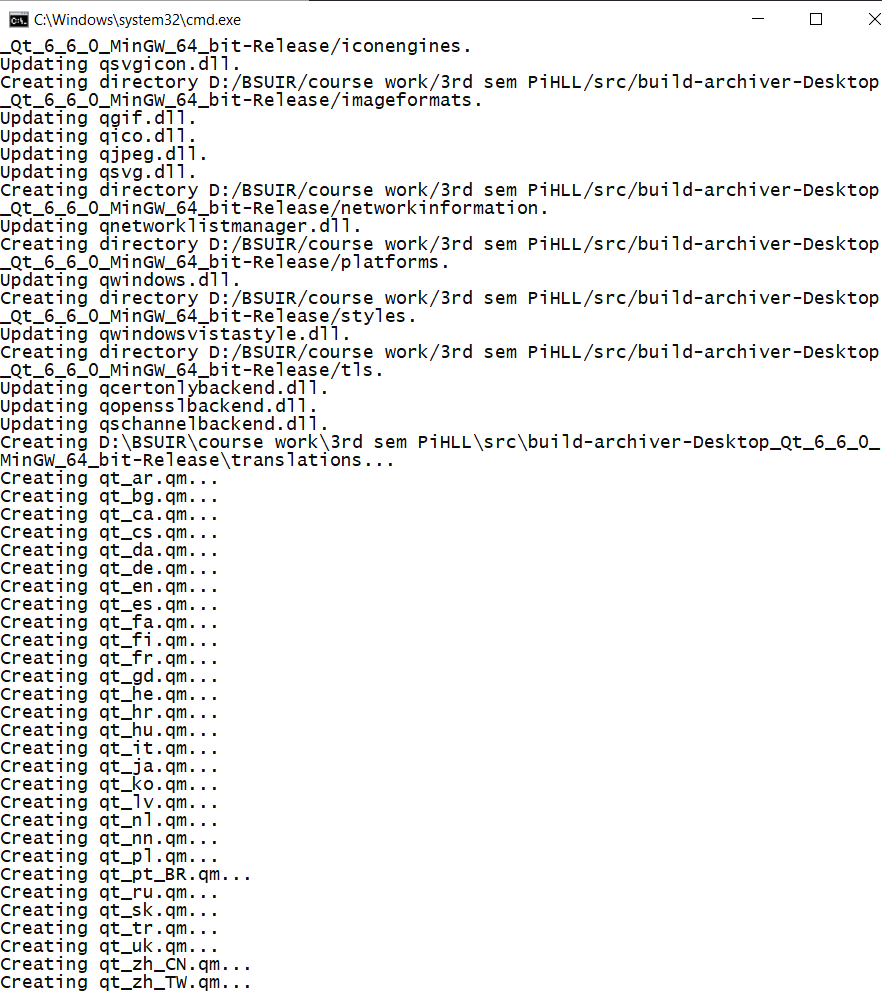
\includegraphics[height=10cm]{\commonSecPathPrefix/sec_5/content/deploy.png}
    \caption{Результат работы утилиты windeployqt.exe}
    \label{fig:deploy}
\end{figure}


Чтобы «отдеплоить» приложения с помощью встроеной утилиты необходимо воспользоваться командной строкой Windows (cmd).
После открытия командной строки используется команда «cd», которая устанавливает текущую директорию содержащую нашу утилиту.
Если директория находится не на диске C, то необходимо перейти в нужный диск.
Например для перехода в диск D необходимо прописать команду «D:».
Потом необходимо прописать название утилиты и через пробел указать полный путь к «.exe» файлу нашего приложения.
Результат работы утилиты можно увидеть на рисунке \ref{fig:deploy}.



После того как приложение было развернуто, им можно полноценно пользоваться.



При открытии приложения по умолчанию пользователю предлагается выбрать рабочий диск.
Далее пользователь выбирает рабочую папку, где он будет взаимодействовать с файлами.
Когда папка выбрана, на левом виджете показывается ее содержимое.

\begin{figure}[h]
    \centering
    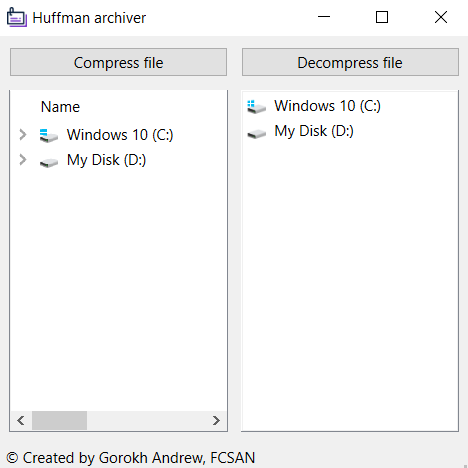
\includegraphics[height=9cm]{\commonSecPathPrefix/sec_5/content/app.png}
    \caption{Оконное приложение Архиватор}
    \label{fig:app}
\end{figure}



Чтобы сжать файл надо нажать на кнопку «Compress file» и выбрать в виджете сжимаемый файл (см. рис. \ref{fig:app}).
После завершения операции на экране высветится сообщение об успешности ее проведения.



Чтобы разархивировать файл необходимо кликнуть по кнопке «Decompress file» и выбрать нужный файл в правом виджете.
Если файл не является архивом, на экран выводится сообщение о невозможности проведения операции разархивирования.
При успешной распаковке создается новый файл с исходными данными и выводится сообщение об успешном разархивировании.



Чтобы открыть файл надо нажать дважды на элемент правого виджета и файл откроется в соответствующем редакторе, предустановленом в ОС для открытия данного типа файлов.